\section{Informatik Grundlagen}

\subsection{Indizierung allgemein}
Bei großen Datenbeständen ist es nicht mehr möglich, die gesamten Daten in den
Arbeitsspeicher unseres Rechners zu laden. Zugriffe auf die Daten sind jedoch nur
vom Arbeitsspeicher aus möglich, wodurch die Daten erst vom Hauptspeicher (z.B. Disk,
HDD, etc.) in den RAM geladen werden müssen, was eine relativ teure Operation ist.
Kommt es hier zu Verzögerungen, so bezeichnet man diese als \textit{Zugriffslücken}.

Daten im Hauptspeicher liegen zumeist nicht als einzelne Objekte vor, sondern als
ganze \textit{Seiten}. Will man nun auf ein Objekt \(a\) auf Seite \(A\) zugreifen,
so muss die gesamte Seite mit allen ihren enthaltenen ELementen mit in den RAM geladen
werden.

\begin{figure}[ht]
	\centering
	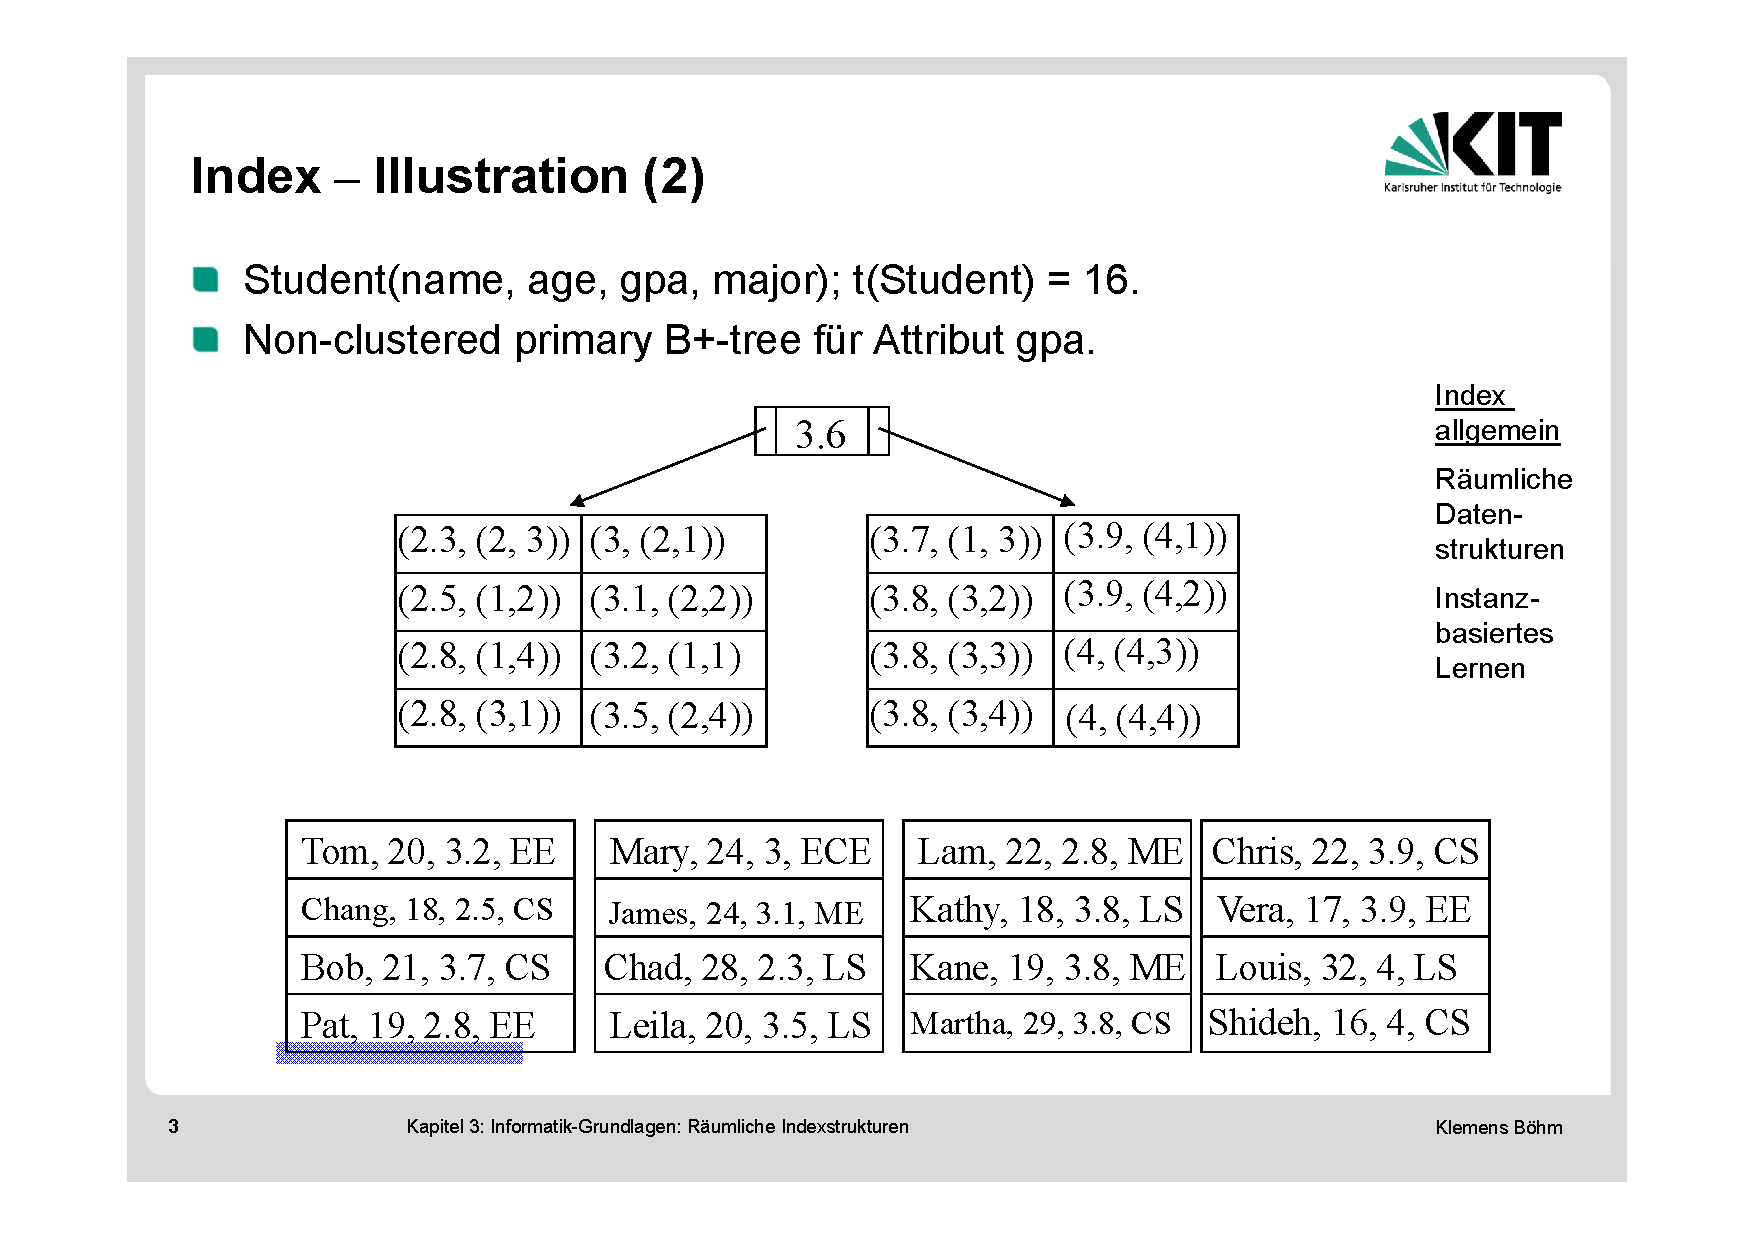
\includegraphics[width=0.75\textwidth]{Figures/index_example}
	\caption[Indizierung Beispiel]{Beispiel für Indizierung eines Seitenweise angeordneten Datenbestandes \footnotemark}
	\label{fig:index_example}
\end{figure}
\footnotetext{3. Foliensatz, S.3, Analysetechniken für große Datenbestände, Prof. Dr.-Ing.
Klemens Böhm}

Dies kann nun ausgenutzt werden, um den Zugriff auf die Daten zu vereinfachen. Betrachten
wir das Beispiel in Bild~\ref{fig:index_example}. Würde man hier z.B. alle Leute
mit einem Notendurchschnitt besser als \(3.6\) ausgeben wollen, müssten aufgrund der
fehlenden Sortierung alle Seiten einzeln in den Arbeitsspeicher geladen werden,
um sich die richtigen Kandidaten heraussuchen zu können; das Problem steigt also
linear mit der Anzahl der Seiten. Liegt hingegen ein
\textbf{Index} vor, hier in Form eines Suchbaumes, so kann die Suche erheblich
vereinfacht werden. Dieser Baum ist dahingehend zu verstehen, dass der erste
Eintrag eines Tupels die Note bezeichnet, nach welcher der Index aufgebaut ist,
und der zweite Eintrag gibt die Seite und die Position auf der Seite des Datensatzes
an. Sucht man nun hier nach allen Leuten, mit einem Notenschnitt besser als \(3.6\),
so erkennt man leicht, dass wir im Baum einfach nach links absteigen müssen. Damit
erhalten wir bereits alle Seiten, die wir in unseren Arbeitsspeicher laden müssen.
Ein effizienteres Beispiel wäre es, wenn wir direkt nach einer bestimmen Note fragen.
Würden wir uns also für den größten Streber interessieren, so müssten wir im Baum
lediglich nach links absteigen und den ersten Eintrag betrachten. Dieser liefert uns,
dass auf Seite 2 an Stelle 3 der Streber \#1 steht. Ohne Index hätten wir alle
Seiten in den RAM laden müssen, um sicher zu gehen, dass nicht auf der letzten
Seite jemand mit einer \(1.0\) auftaucht.

Diese Indizierung ist natürlich auch für \textbf{mehrere Attribute} möglich.
Oben kommt die Note \(3,8\) mehrfach vor. Sortieren wir zusätzlich auch nach dem
Namen, erhalten wir eine eindeutigere Indizierung. Es gilt zu beachten, dass
eine Sortierung \((gpa, name)\) im Allgemeinen \underline{nicht} \((name, gpa)\)
gleicht.

\subsection{Räumliche Indexstrukturen}
\subsubsection{Normalisierung}
Betrachten wir nun Datenbestände mit mehreren Dimensionen. Möchte man hier die
Ähnlichkeit von zwei Datensätzen bestimmen, so wäre ein naiver Ansatz, einfach
die Distanz zwischen den beiden Punkten im \(n\)-dimensionalen Raum zu berechnen.
Ein Problem ergibt sich jedoch daraus, dass mit der einfachen Berechnung des Abstandes
zweier Punkte der sich ergebende Wert mit der Anzahl der Dimensionen automatisch
mitwächst. Deswegen ist eine Normalisierung nötig. Im zwei-dimensionalen Raum mit
jeweils unterschiedlichen Einheiten würde dies mittels
\[
	a_i = \frac{v_i - min\ v_j}{max\ v_j - min\ v_j}
\]
geschehen, wobei \(v_i\) ein Wert aus dem betrachteten Tupel ist (ob es der erste
oder zweite Wert ist, spielt keine Rolle, beide werden gleich normiert) und \(v_j\)
ein anderer Wert aus dem Wertebereich ist. Die Notation ist tatsächlich nicht schön.

Diese Normierung trägt zwar den Unterschieden in den Einheiten der Dimensionen
Rechnung (z.B. Alter und Einkommen), jedoch noch nicht der Anzahl der Dimensionen.
Würde man nun einfach den Abstand der Punkte berechnen, ergäbe sich mit
\[
	d(x_1, x_2) = \sum\limits_{i\in D} |x_{1,i} - x_{2,i}|
\]
die sogenannte \textit{Manhatten Distance}. Mit dieser Formel ist die Abhängigkeit
des Abstands von den Dimensionen eindeutig. Um diese nun auch zu normieren, gibt
es die \textbf{Manhatten Segmental Distance} mit
\[
	d_D(x_1, x_2) = \frac{\sum\limits_{i\in D} |x_{1,i} - x_{2,i}|}{|D|}
\]
wobei \(|D|\) die Anzahl der Dimensionen ist.

\subsubsection{k-dimensionale Bäume}
Das Konzept von kd-Bäumen ist einfach erklärt. Man nehme eine Dimension und suche
sich den Punkt, bei welchem die Hälfte der Datensätze jeweils auf beide Seiten
verteilt ist. Nun nehme man die nächste Dimension, und wiederholt das Ganze. Dieses
Spiel wird nun so lange getrieben, bis man entweder jeden Punkt eindeutig durch
einen Pfad beschrieben hat, oder in jedem Blatt nur noch ein gewisse (geringe) 
Anzahl an Elementen liegt. Auf diese Weise kann man Punkte durch Traversieren
des Baumes sehr leicht auffinden. Auch sind Bereichsanfragen möglich. 
Im 2D-Raum würde dadurch eine Art "'Raster"' entstehen.
\textit{Bereichsanfragen} sind möglich, indem man prüft, ob der Raum, den man abfragt
eine Überlappung mit dem Split des aktuellen Knotens hat, oder nicht. Fall
der Bereich nur in eine Hälfte des Splits fällt, dann kann man einfach in diesen Teilbaum
absteigen und den anderen Teilbaum vernachlässigen. Fällt ein Split jedoch
in den Bereich der Anfrage, so muss man in beide Teilbäume absteigen, um alle
Elemente in diesem Bereich finden zu können.
Die \textit{Nächster Nachbar Anfragen} haben den Vorteil, dass nicht jeder Datenpunkt
einzeln verglichen wird, sondern nur die von bestimmten Zonen, die durch den
kd-Baum gegeben sind. In Algorithmus~\ref{alg:NN} ist ein beispielhafter Algorithmus
für eine NN-Anfrage mit einem kDB-Baum gegeben.

\begin{algorithm}[htb]
	\SetAlgoLined
	\DontPrintSemicolon
	\SetKwInOut{Input}{input}\SetKwInOut{Output}{output}
	\BlankLine
	\Input{K-D-B-Tree, Query}
	\BlankLine
	\ {Queue := new Priorityqueue()}\;
	\ {Region := Root}\;
	\ {Distance := Dist(Region, Query)}\;
	\ {Enqueue(Queue, Distance, Region)}\;
	\BlankLine
	\While{true}{
		Element = Dequeue(Queue)\;
		\eIf{Element is object}{
			\Return{Element}
			}{
			\eIf{Element is leaf}{
				\ForAll{objects in Element}{
					Distance = Dist(object, Query)\;
					Enqueue(Queue, Distance, object)\;
					}
				}{
				\ForAll{Child of Element}{
					Distance = Dist(Child, Query)\;
					Enqueue(Queue, Distance, Child)\;
					}
				}
			}
		}
	\BlankLine
	\Output{Nearest Neighbor}
	\caption{Algorithmus für eine NN-Anfrage mittels eines kDB-Baumes.\label{alg:NN}}
\end{algorithm}


Die genaue Berechnung der Distanzen des Anfragepunktes zu den Zonen ist im Einzelnen
zu implementieren, je nach gegebenem Fall.

\subsubsection{Objekte mit räumlicher Ausdehnung}
Im Folgenden sollen die zu untersuchenden Objekte nicht nur lediglich durch Punkte
dargestellt werden, sondern auch durch höher-dimensionale Objekte. Diese Objekte
können z.T. nicht regelmäßig sein, was die Arbeit mit diesen Objekten deutlich
erschweren kann. Deswegen können diese durch die so genannten \textit{Minimum
Bounding Rectangles} approximiert werden, welche man sich als Box kleinster
Ausdehnung vorstellen kann, die das Objekt noch umfasst. Mit solchen Objekten
stellt sich für Punktanfragen die Frage, in welche der Objekte (Rechtecke) der
Punkt fällt. Die Rechtecke können sich durchaus auch überschneiden und überlappen
und sie werden durch eine bestimmte Menge an Punkten beschrieben. Im 2-dimensionalen
sei dies \((links,\ rechts,\ unten,\ oben)\), also x-Position links /rechts und 
y-Position oben / unten. 

Auch hier lässt sich der Raum an bestimmten Werten splitten und als Baum
repräsentieren. Im 2-dimensionalen Fall würde man also nach den einzelnen
Seiten der Rechtecke splitten. Der Unterschied zu normalen kd-Bäumen besteht
hierbei jedoch darin, dass, wenn der zu suchende Punkt zum Beispiel einen größeren
x-Wert aufweist, als der aktuelle Schwellenwert
für die linke Seite, man nicht nur in den rechten
Teilbaum absteigt, sondern man in beide absteigen muss. Insbesondere gilt es zu
beachten, dass dies jeweils für die zu untersuchende Seite der Rechtecke gilt,
d.h. würde man nun nach dem x-Wert der rechten Seite unterscheiden, so müsste man
in beide Teilbäume absteigen, wenn der Wert des zu suchenden Punktes kleiner als
der Schwellenwert wäre. Entsprechendes gilt auch für die oberen und unteren
Seiten. 

\subsubsection{Optimierung kd-Bäume}
Zunächst eine Klarstellung: \textit{Physische Knoten} sind die Seiten auf dem
Speichermedium, \textit{Logische Knoten} sind die Knoten des Baumes. Nach dieser
Interpretation ist es durchaus möglich, dass ein physischer Knoten mehrere logische
Knoten enthalten kann. Es wäre auch verschwenderisch, jeden logischen Knoten durch
eine Seite im Speicher zu repräsentieren. 
Die kompakte Darstellung der Knoten erlaubt es, mehrere logische Knoten auf einer
Seite zu speichern. 

Außerdem kann es durch die Wahl der Splits
zu einem sehr unbalancierten Baum kommen. Effizienter wären die Anfragen dann,
wenn der Abstand der einzelnen Datenpunkte zur Wurzel immer gleich wäre, der 
Baum also balanciert ist. Hierfür nutzen wir aus, dass ein physischer Knoten
auch mehrere logische Knoten enthalten kann, und damit in Folge auch mehrere 
logische Regionen enthalten kann. Logische Regionen sind bestimmmte Wertebereiche
der Datenpunkte.


\begin{figure}[htbp]
	\centering
	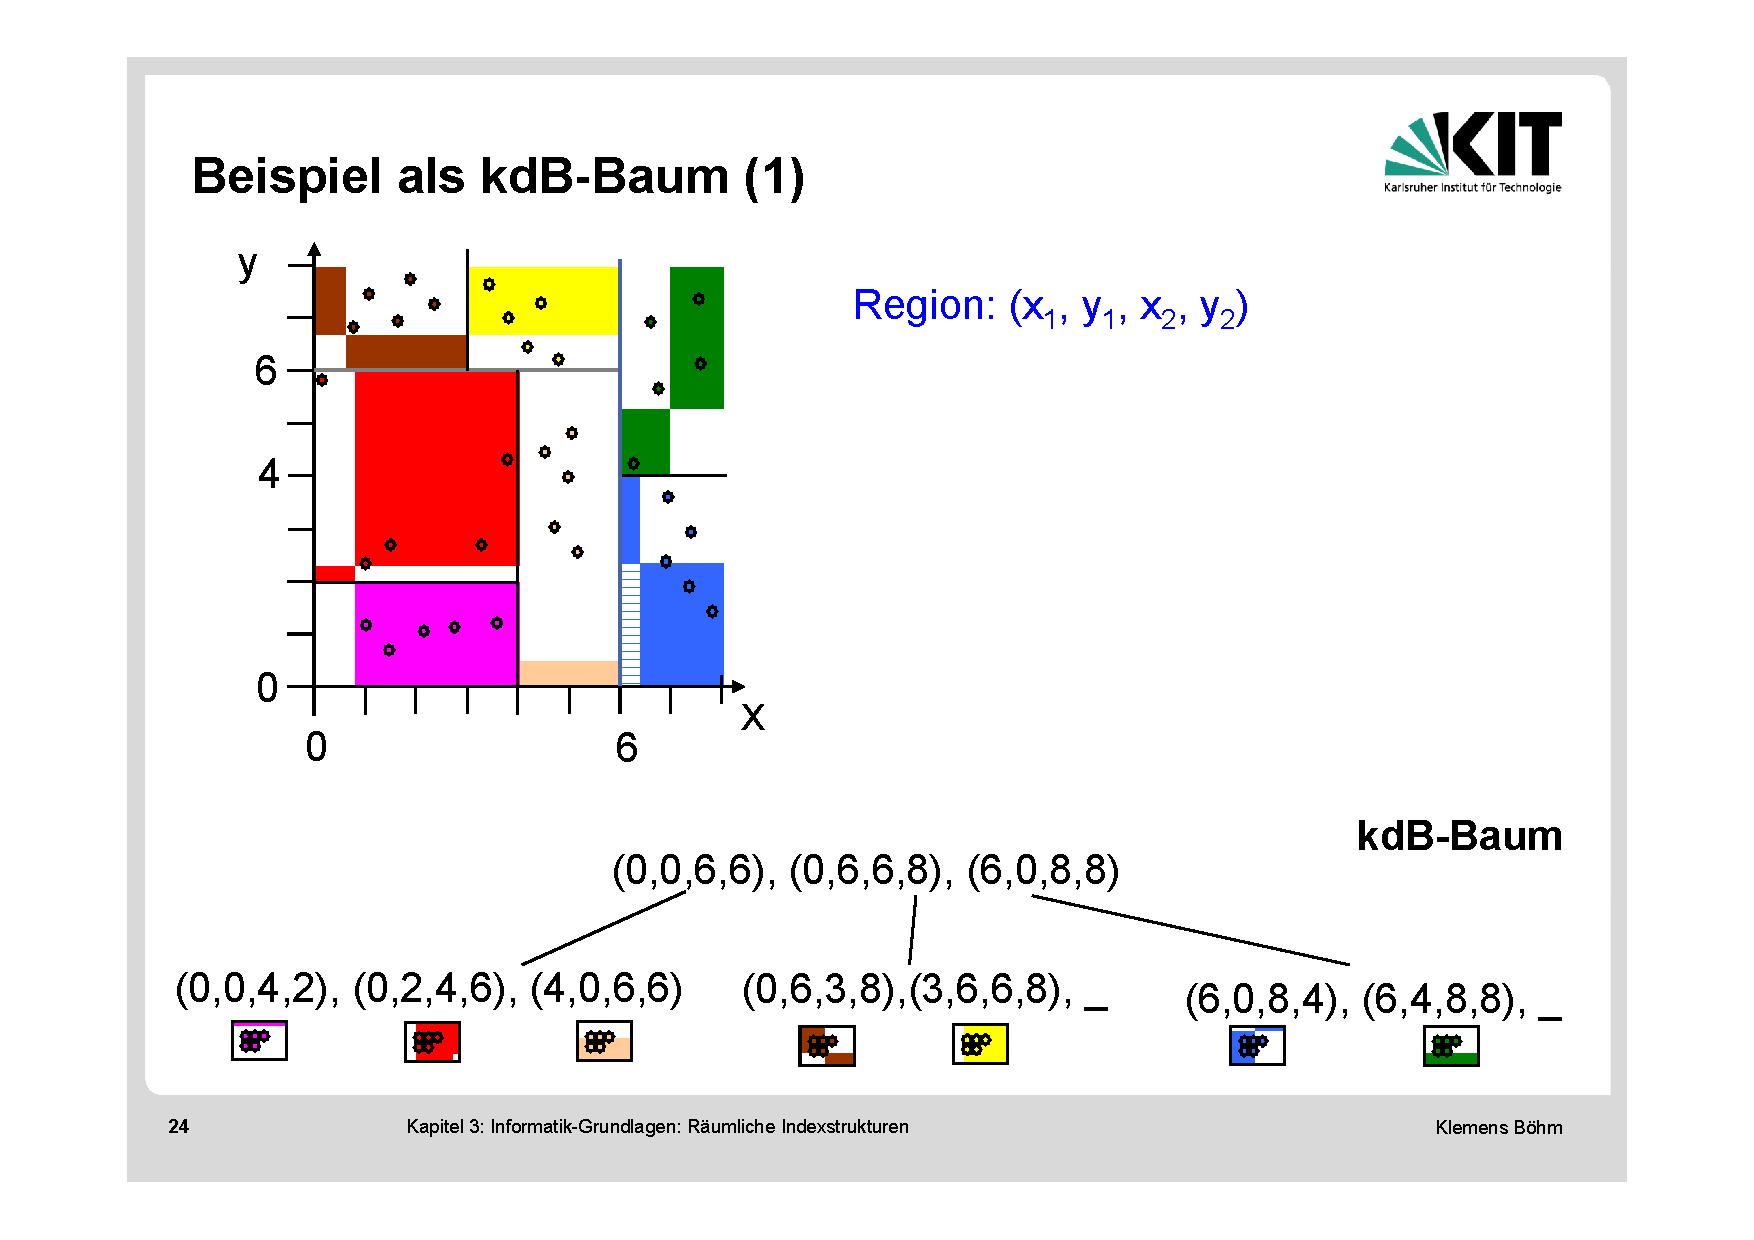
\includegraphics[width=0.75\textwidth]{Figures/kdB_Tree}
	\caption[kdB-Baum]{Optimierung eines kd-Baumes durch Kombination mit einem B*-Baum}
	\label{fig:kdB_Tree}
\end{figure}
\footnotetext{3. Foliensatz, S.24, Analysetechniken für große Datenbestände, Prof. Dr.-Ing.
Klemens Böhm}

In Abb.~\ref{fig:kdB_Tree} ist beispielhaft ein so genannter kdB-Baum dargestellt.
Die verschiedenen logischen Regionen sind farblich gekennzeichnet. Sie entsprechen
einfach dem Beispiel des kd-Baums aus der Vorlesung. In einem kd-Baum
haben die Knoten die Splitdimensionen dargestellt, hier stellen die Knoten jetzt 
verschiedenen logischen Regionen dar.
Diese logischen Regionen müssen nicht unbedingt den elementaren Partitionen
(also den einzelnen Farben) entsprechen, sondern können auch mehrere 
zusammenfassen. Dadurch geben die Knoten, wenn man sie als logische
Hierarchie auffasst, nicht die Partitionierungsstruktur wieder, wie es der kd-Baum
getan hat. Die einzelnen Knoten, bzw. ihre Elemente (z.B. (0,0,6,6)) beschreiben
nun aber einen größeren Ausschnitt des Raumes, und das auf kompakte Weise.
Der Baum der entsteht ist augenscheinlich balanciert; nutzt man diese Balance aus,
indem man nun den einzelnen Knoten ihre eigenen physischen Seiten im Speicher
zuweist, so ergibt sich eine balancierte Suchstruktur auf Speicherebene. Das ermöglicht eine
verbesserte Performance.
Für die Prüfung sollte man wohl lediglich die Vor- und Nachteile eines kdB-Baumes
kennen.

\begin{table}[thbp]
\begin{tabular}{p{5cm} l}
	\toprule
	Vorteile & Nachteil \\
	\midrule
	Abstand Daten und Wurzel immer gleich & Komplexe Reorganisation \\
	\midrule
	Pro physischem Knoten genau eine Speicherseite & \\
	\midrule
	Effizienterer Zugriff & \\
	\bottomrule
\end{tabular}
\end{table}

\subsubsection{R-Baum}
Der \textbf{R-Baum} ist eine ebenfalls balancierte Indexstruktur, die schnelle Suche nach und
auf Objekten mit räumlicher Ausdehnung erlauben. Realisiert wird dies, indem
in den Blattknoten nur die Datenobjekte enthalten sind und in den übrigen Knoten
so genannte \textit{minimum bound rectangles} gespeichert werden. Diese Rechtecke
enthalten alle im darunter liegenden Teilbaum befindlichen Datenobjekte. Datenobjekte
können entweder Datenpunkte, rechteckige Bereiche oder Polygone sein, wobei letztere
meist durch ein Rechteck approximmiert werden.

\begin{figure}[ht]
	\centering
	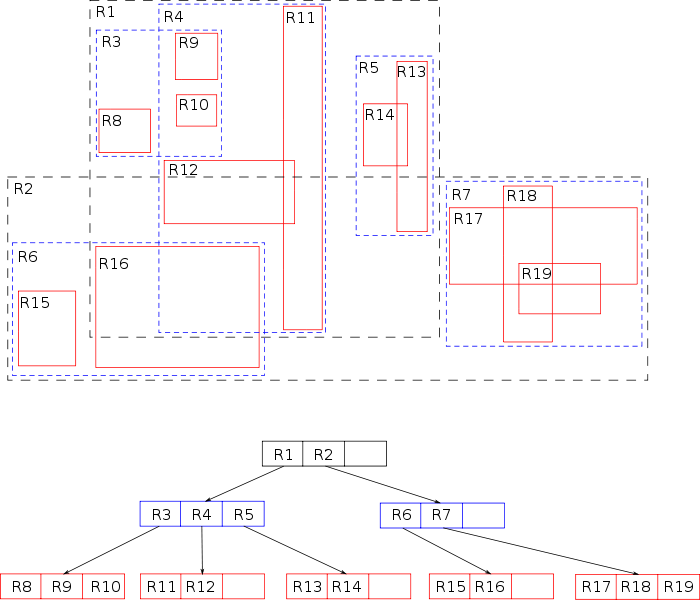
\includegraphics[width=0.75\textwidth]{Figures/r_tree}
	\caption[R-Baum 2D]{Beispiel für einen R-Baum und Visualisierung der
	räumlichen Indizierung.\footnotemark}
	\label{fig:r_tree}
\end{figure}
\footnotetext{https://upload.wikimedia.org/wikipedia/commons/6/6f/R-tree.svg}

\begin{figure}[ht]
	\centering
	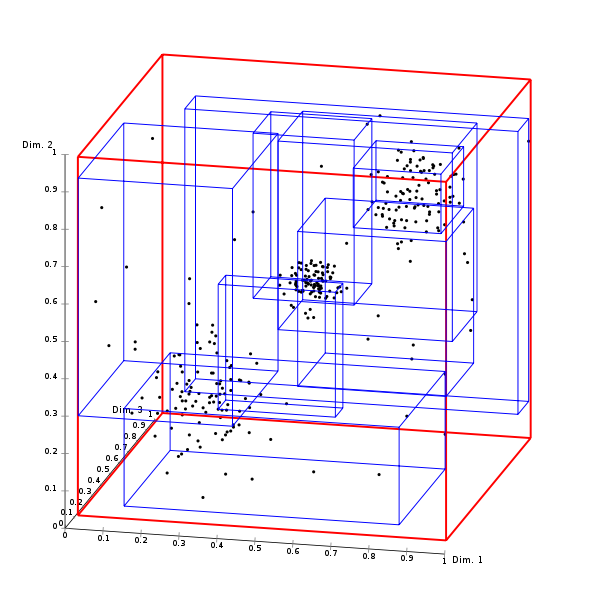
\includegraphics[width=0.75\textwidth]{Figures/r_tree3D}
	\caption[R-Baum 3D]{Beispiel für einen 3D-R-Baum.\footnotemark}
	\label{fig:r_tree3D}
\end{figure}
\footnotetext{https://upload.wikimedia.org/wikipedia/commons/5/57/RTree-Visualization-3D.svg}

Der Vorteil eines R-Baums besteht darin, dass bereichsspezifische Anfragen effizient
beantwortet werden können, ob z.B. der Anfragebereich in einem bestimmten Rechteck
enthalten ist, oder welche Rechtecke im Anfragebereich liegen. Auch die NN-Anfrage
kann effizient bearbeitet werden,
sofern die Distanzen in Rechecke umgewandelt werden können.
Außerdem ist ein R-Baum \textit{dynamisch}, er 	kann also laufend
aktualisiert und erweitert werden. Beim \textit{Einfügen} kann im Wesentlichen
zwischen 3 Fällen unterschieden werden. 

\begin{itemize}
	\item Punkt fällt in Zone \textbf{genau eines Kind-Knotens}: Es wird einfach naiv
		in den entpsrechenden Knoten eingefügt.
	\item Punkt fällt in \textbf{Überlappung} von 2 Kindknoten: Optimale Entscheidung ist
		sehr schwierig zu treffen bis unmöglich ohne weitere Hinweise.
	\item Punkt fällt \textbf{außerhalb} jeder Zone: Es wird der Punkt in den Knoten
		eingefügt, durch den die Vergrößerung der Rechtecksflächen minimal
		bleibt.
\end{itemize}

Beim Einfügen kann es nun passieren, dass irgendwann in einem Blattknoten zu
viele Kinder enthalten sind. Um dem entgegenzuwirken gibt es den
\texttt{LinearSplit}, welcher zunächst alle Datenobjekte in dem betroffenen Blatt
auf ihre Distanz zueinander untersucht und das Paar mit dem größten Abstand
auswählt. Die beiden gewählten Objekte dienen nun jeweils aus Ausgangspunkt für
die Erzeugung der beiden neuen Blätter. Es werden die übrigen Objekte nun derart
auf die neuen Blätter verteilt, dass der Zuwachs der Fläche jeweils möglichst gering
ausfällt. Da die Reihenfolge der Betrachtung der Blätter nicht fest vorgeschrieben
ist, kann es bei mehreren Durchläufen des selben Splits zu unterschiedlichen
Ergebnissen kommen.  Es sei angemerkt, dass es noch weitere Ansätze für den
Split gibt, die jedoch aufgrund ihrer quadratischen bzw. exponentiellen Laufzeit
in der Mächtigkeit der Menge der Datenobjekte und dem nur geringen Qualitätszuwachs
des Ergebnises in der Realität fast nie Anwendung finden. 
Im Übrigen sind auch R-Bäume nicht vom Fluch der Dimensionalität befreit. Durch
zu viele Dimensionen kommt es zu immer häufigeren Überlappungen der Objekte,
wodurch die Effizienz der Suche stark leidet, da nun nicht mehr eindeutig ist,
in welchen Teilbaum man absteigen muss.

Als Schlusswort zum R-Baum wie zu allen oben genannten Indexstrukturen lässt
sich festhalten, dass sie alle nur einen Kompromiss darstellen. Zwar wird das
Auffinden der Datenobjekte durch die Indizierung erheblich effizienter, die
Verwaltung und die Aktualisierung der Strukturen ist jedoch um einiges komplexer
als das naive Speichern der Daten. Im Gegenzug für die höheren Anforderungen an
Speicherverbrauch und Rechenzeitbedarf bei Änderungen erhält man meist sehr effiziente
Zeiten bei Suchanfragen.


\subsection{Instanzbasiertes Lernen}
Das \textbf{Instanzbasierte Lernen} ist im Maschinellen Lernen ein Verfahren, dem
das Prinzip der \textit{NN-Anfrage} zugrunde liegt. Bei anderen Methoden des
Maschinellen Lernens geht es zumeist darum, dass mit Hilfe eines Trainingsdatenbestandes
ein Modell erzeugt wird, dass zur Vorhersage der Klasse eines unbekannten Objektes
verwendet wird. Beim Instanzbasierten Lernen, auch "'Lazy Learning"', entfällt
dieser Schritt, denn es wird beim Untersuchen eines unbekannten Objektes der
Trainingsdatenbestand direkt zu Rate gezogen. Das heißt, es wird mit dem neuen
Objekt eine NN-Anfrage auf dem Trainingsdatenbestand ausgeführt, und das Ergebnis
bestimmt dann die Klasse des neuen Objektes. Offensichtlich kann es durch Rauschen im
Trainingsdatenbestand zu Fehlentscheidungen kommen, wenn lediglich der nächste Nachbar
gesucht wird. Eine \textit{k-NN-Anfrage} kann hierbei Abhilfe verschaffen, da nun die
\(k\) nächsten Nachbarn untersucht werden und damit das Rauschen herausgefiltert werden
kann.

Der Vorteil von Instanzbasiertem Lernen liegt darin, dass der hohe und komplizierte
Arbeitsaufwand für die Modellerstellung entfällt. Dafür muss jedoch bei jeder
Entscheidung eine NN-Anfrage auf dem Trainingsdatenbestand ausgeführt werden, was
signifikant ineffizienter ausfällt, als Modellentscheidungen. Dafür kann jedoch auch
gut mit sich ändernden Datenbeständen umgegangen werden, indem einfach schnell der
Trainingsdatenbestand angepasst wird. Außerdem hat jedes Attribut den gleichen Einfluss
auf das Resultat. Bei Modellbasiertem Lernen können die Attribute unter Zunahme
von Domänenwissen priorisiert werden. Ganz pragmatisch sei hier die Kostenabschätzung
für ein zu bauendes Haus gennant: Faktoren wie die Anzahl der Stockwerke und 
Unterkellerung haben offensichtlich einen größeren Einfluss auf die Kosten als
die Lage und Größe des Grundstücks.

Die Anwendung eines Suchbaumes als Indizierung für den Trainingsdatenbestand ist
hierbei unumgänglich. Auch hier kann es jedoch zu den üblichen Problemen bei zu
hoher Dimmensionalität kommen. So kann es bei Indexstrukturen über hochdimensionierte
Daten zu Problemen mit der Aussagekraft der Distanzwerte kommen oder es kann aufgrund
der Anzahl der Dimensionen zu viele Partitionsmöglichkeiten geben.

